\chapter{Temporal Side Channels Part 2} \label{cha:Temporal Side Channels Part 2}

\section{recap}\label{sec:recap}

In the previous chapter we discussed about RSA cryptosystem~\cite{wikiRSA}, and presented  the most expensive operation in the RSA. When we need to take the message (m) and raise it to the power of the key (either the public key, the private key, the verification key and so on)
\[ C = m^e(modn) \]
But the simplest algorithm to raising by a number uses modular multiplication which is an expensive operation.

\begin{figure}[!ht]
    \centering
    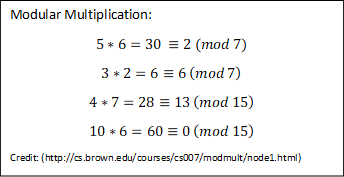
\includegraphics{images/modmul.png}
    \caption{Modular multiplication} \label{fig:modmul}
\end{figure}

Modular multiplication is pretty straightforward. It works just like modular addition. You just multiply the two numbers and then calculate the standard name. Examples for Modulo 7 and 15 can be found in \Cref{fig:modmul}. Why modular multiplication is expensive? Because we have to take the modulo many times which is as expensive as division. Division is the most expensive integer operation exists, and  therefore we don't want to do many divisions. So, one way to do this is by multiplying and multiplying and doing the modular reduction at the end, but the problem is the runtime of multiplication grows exponentially with the number of the multiplicands. 
Other way is with each multiplication do a  \( mod n \), but the numbers grow longer and longer, and the runtime gets higher and higher, so we can't do that either. 

\begin{figure}[!ht]
    \centering
    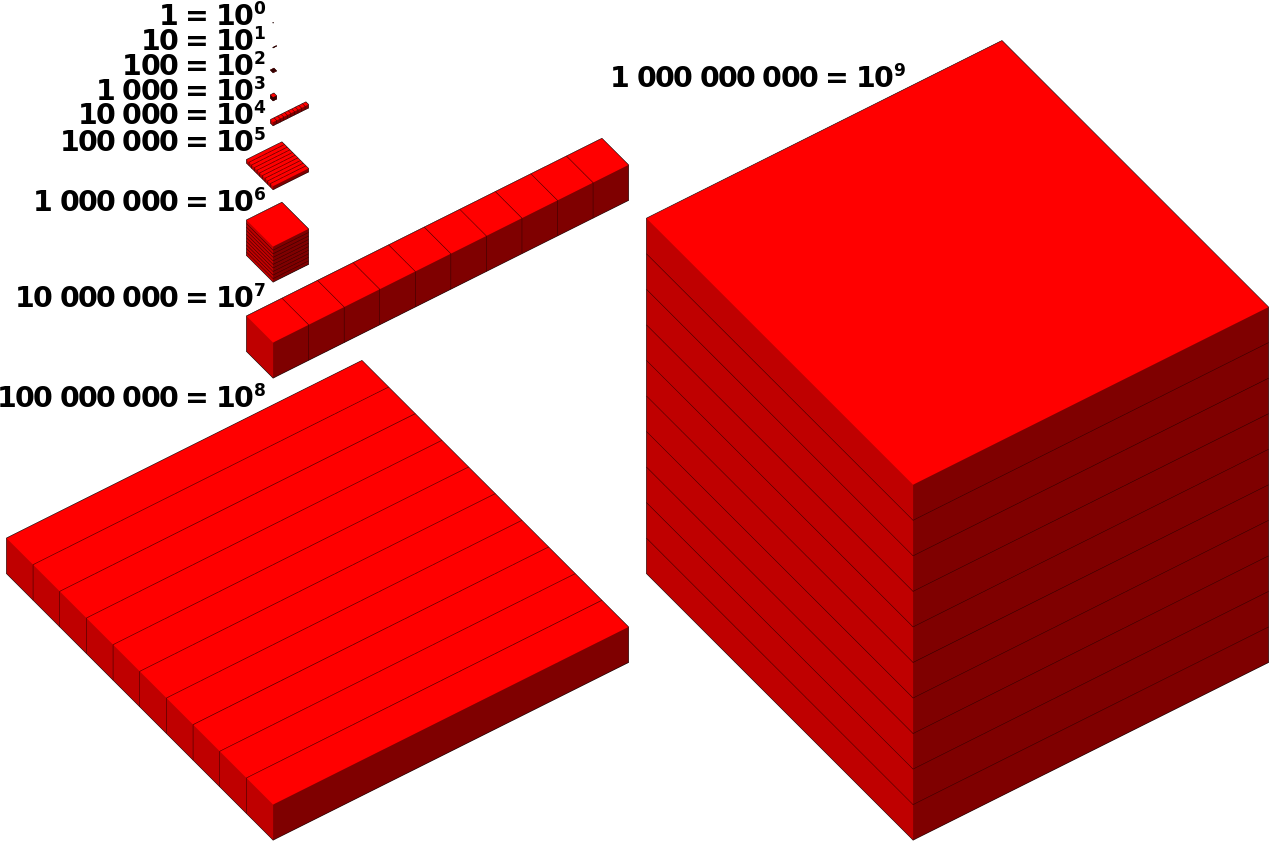
\includegraphics[scale=0.25]{images/vispow10.png}
    \caption{Visualization of powers of 10 from one to 1 billion.} \label{vispow10:fig}
\end{figure}

So, as we discussed in the last chapter, the slowest and most trivial way of implementing modular multiplication is just to take $g$ and multiply it by $g$, by $g$, by $g$ ($e$ times) \(g^e mod n\) and every once in a while doing modulo n, either every multiplication or just in the end. The problem with this was that if e is a number that consists of 1024 bits, then the worst case number that we might need to multiply $g$ is \( 2^{1024} \) which is a lot, we don't want to do that.

\section{Efficiently Implementing Modular Exponentiations}\label{sec:Efficiently Implementing Modular Exponentiations}

There are two ways of making this faster, and these two ways are either performing fewer modular multiplication (instead of  \( 2^{1000} \)  we would like to do 1000) and we also want the modular multiplication to be less expensive. The best case, would be same as regular multiplication over integer. These two ways will reduce the cost of modular multiplication and modular exponentiations, and this is something we really want to do to make RSA work on a device.

So, assume we are engineers, we want to implement modular exponentiations very cheaply. The right thing to do is of course to use some crypto library, but let's assume that's not possible, we are inventing the new CPU or something. So, there is very serious book online called the handbook of applied cryptography (\Cref{fig:appliedCrypt})~\cite{katz1996handbook}. The book is like a phone book or a recipe book, and is filled with algorithms, proofs and equations you need for cryptography. Chapter 14 deals with efficient algorithms for multiplicative proofs. The book contains the ways to do modular exponentiation: very cheaply, more cheaply and the old fashion approach. 

\begin{figure}[!ht]
    \centering
    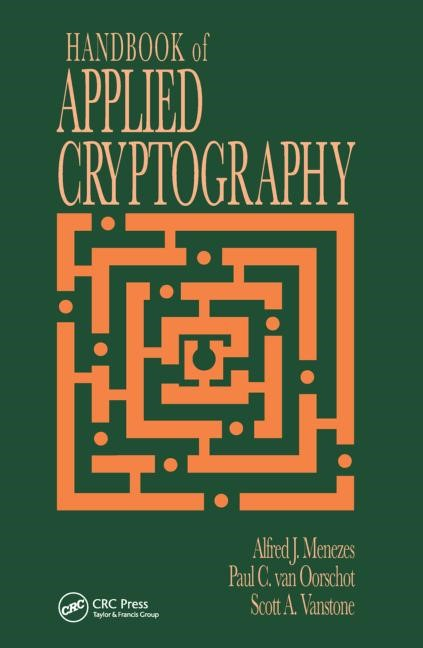
\includegraphics{images/appliedCrypt.jpg}
    \caption{Cover of the handbook of applied cryptography} \label{fig:appliedCrypt}
\end{figure}

The following approach is called the left to right binary exponentiation, also known as square multiply.
\begin{figure}[!ht]
    \centering
    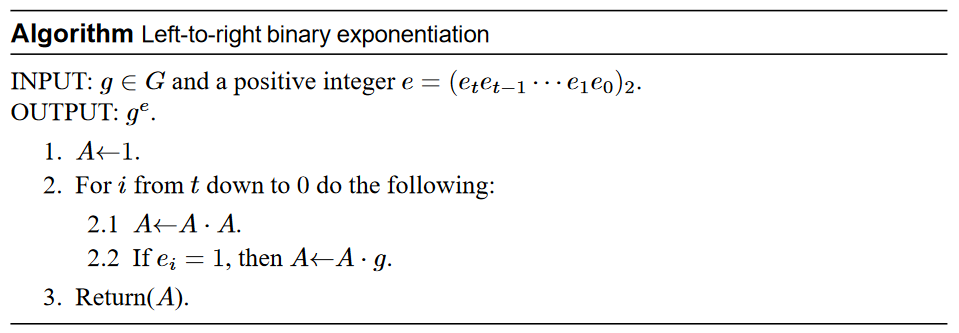
\includegraphics[scale=0.4]{images/ltrbe.png}
    \caption{The pseudo-code was taken from the handbook of applied cryptography, page 615.} \label{fig:ltrbe}
\end{figure}

The inputs are $g$ (we want to raise g to the power of $e$, \(g^e\)) and \(e\) which is a bit string of $t$ ($t$ bits), in the book its $t+1$ (see \Cref{fig:ltrbe}). The most significant bit is always $1$, because there is no logic behind raising something to the power of zero. In this algorithm in the end \(A\) will be the result of $g$ raised to the power of $e$. 

In the beginning we set $A$ to be equal to $1$, and go over the bits from left to right (from the most significant to the least). Each time we do square ($A$ equal $A$ times $A$, $A=A*A$) and multiply but we don't always multiply, we do it sometimes. If the current bit is $1$ (the \( i^{th}\) bit) then we multiply by $g$, $A=A*g$. This is the algorithm. Now, what happens when we do a squaring operation downstairs? What happens to the exponent upstairs? Its multiplied by $2$. So \({g^{e}}^2 = g^{2e} \)  and  \(g*g^{e} = g^{e+1} \). Now, we can think of a binary string, you can write down the bits using shifting (multiplying by $2$ is shifting) and adding $1$ is just putting one in the place.

So how many modular multiplications will be performed in order raise g to the power of $e$ (the string is of length $t$)? The answer is \(O(t)\) What is the base case - lowest amount of multiplication that will be performed? the answer is $t+1$, the first bit is $1$ (most significant) so we do step 2.2 one time and all the rest of the string is zeros, and each time we do step 2.1. What is the  highest amount of multiplication that will be performed? Answer: $2t$, if all the bits $1$ I do each time $2$ multiplications (step 2.1 and step 2.2). Anyway, this is \(O(t)\).

So, instead of \(2^t\) as in the old algorithm we performed at most $2t$ multiplications. 

Lets review an example. Lets calculate \(7^6=7^{(110)}\) in the group \( \mathbb{Z}_{15}={1, 2, 4 ,7, 8, 11, 13, 14} \).

\begin{enumerate}
	\item  \(A = 1 = 7^(0) \)
	\item  \(A = A*A = 1 = 7^{(0<<1)} = 7^{(0)}\)
	\item  \(A = A*7 = 7 = 7^{(0+1)} = 7^{(1)}\)
	\item  \(A = A*A = 4 = 7^{(1<<1)} = 7^{(10)} \)
	\item  \(A = A*7 = 13 = 7^{(10+1)} = 7^{(11)} \)
	\item  \( A = A*A = 4 = 7^{(11<<1)} = 7^{(110)} \)
\end{enumerate}

Are there any ways doing it even faster? the answer is yes we can open the handbook of applied cryptography and find some others.
The general thought of these algorithms is that we do some precomputation. In RSA there is a public number that you know that you are going to start, so g is known number, we don't care what $g$ is. So if we know what g is we can prepare all sort of lookup tables, in the window method we take each time three bits at the same time, and instead of doing \(A*g\) we do\( A*g*g\) or \(A*g*g*g\) .. (8 values we can use), and instead of \( A=A*A\) we do \(A=A*A*A\) and so on, this is the sliding window. There is binary method, you can just look at the book and find out (page 616 algorithm 14.83, in the handbook of applied cryptography). So this is how you reduce modular multiplications and we can assume that any reasonable crypto implementation is not doing the naive method. It will use the left to right or the right to left which is basically the same idea or one of the window methods.

But what if we want the modular multiplication to be cheaper? There is a way and it's called the Chinese remainder theorem (CRT)~\cite{dingyi1996chinese}, which is called after Sun Tzu Suan, that was a teacher from the \nth{5} century and he wrote a book that contained all sorts of riddles and questions. And there is the riddle: 

``there are certain things whose number is unknown.  If we count them by threes we have two left over; by fives we have three left over; and by sevens, two are left over. How many things are there?" 

The answer is 23 and how it was discovered? Brute-force.
So the CRT states that you have to have an equation set over modulo other multiplicative group such as this, you can solve it modulo $p$, you can solve it modulo $q$, this is more general theorem. You can solve it modulo the underling primes then combine them, and if there is only one solution in each of the sub-groups there is only one solution in the big group. What this means is that if we want to do modular multiplication in this big field modulo $N$, we can actually do the computation in modulo $p$ and modulo $q$ and then we can combine them together. Why does this help us (we have to do 2 operation instead of one)? Answer: to do exponentiation in CRT we take our  big number and do modulo $p$ and again modulo $q$ and then there is a CRT step. So these two modular exponentiations, what is the size of the operand they are using? Assuming that $p$ and $q$ are of the same size? Let's say $p$ and $q$ is 1000 bits so the size of $n$ is 2000 bits (we add the number of bits of each number in the multiplication).  So each number in the multiplicative group is about 2000 bit because its mod $N$, so multiplying two numbers is going to be multiplying two numbers which are 2000 bits. If we reduce it to modulo $p$ and modulo $q$ my numbers are going to be half the size (1000 bits). So if we take a multiplication and now we will multiply two number that are half the bit length what is the speed improvement I get? It's times 4. Instead of one modular exponentiation we have one baby modular exponentiation which costs me quarter of the time and another one which cost me quarter of the time and a step (the CRT step which is a modular multiplication of the two). How much we spent in total? Answer: a bit more than half the time, twice speedup. Why can't we do that further? Divide $p$ and do it again? Answer: because it's a prime number ($p$ and $q$) that's the whole point. So if you do the CRT each modular exponentiation will take less time. 

Now there is a really nice trick, to make modular multiplications very cheap and this actually makes modular multiplications as cheap as regular multiplication. So, magic, what is the problem? Multiply two number is pretty easy but the problem is reducing after multiplying. So what if there is a way of doing modular multiplications without the reduction step? So in 1985 a genius mathematician called peter Montgomery published a paper called ``modular multiplication without a reduction step" ~\cite{warren2013hacker}\footnote{https://www.hackersdelight.org/MontgomeryMultiplication.pdf}. So the idea is there is a kind of magical world called the Montgomery representation and you take your number and you step into the Montgomery world where modular multiplications do not require reducing step and when you finish you step out of this world and you are back with your result. It's still cost you like a multiplication but it doesn't cost you the extra reduction step.
So, what is the idea of the Montgomery reduction? we want to calculate \(g^emodn\) and to do that we need to pay a lot of modular reduction which we  don't want. So, the first thing we do is enter the Montgomery representation and we do the Mont(\(g^e\)) and each one of this multiplication steps is going to be about as difficult as regular multiplication (Figure Figure \ref{montg:fig}). When we  finished with this we exit the Montgomery representation and then we have our result. Entering and leaving the Montgomery representation costs as much as modular multiplication but in the middle it's as cheap as regular representation.

\begin{figure}[!ht]
    \centering
    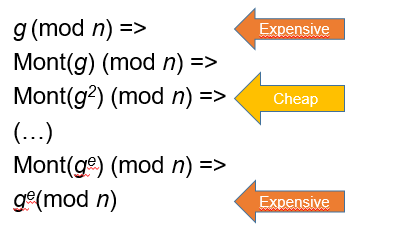
\includegraphics[scale=0.7]{images/montg.PNG}
    \caption{General sketch of Montgomery Exponentiation} \label{montg:fig}
\end{figure}

Now lets review how the Montgomery Exponentiation works inside
\begin{enumerate}
	\item  Choose a value R, \(R>n\), which is easy to use (usually a large power of 2)
	\item  \(Mont(a)=a*R(mod n) =^{def}  a(mod n)\)
	\item  \(Mont(ab)=a*b*R(mod n)=\underline{a}*\underline{b}*R^{-1} (mod n)\)
	\item  \(... \)
	\item  \( = (\underline{a}*\underline{b} + (\underline{a}*\underline{b}*n'(mod R)*n))/R(modn) \) \newline
	// if this is more than n, subtract n
	\item  \( A = A*A = 4 = 7^{(11<<1)} = 7^{(110)} \)
	\item  Result: Instead of modular reduction, we only (sometimes) subtract
\end{enumerate}

The first thing to do is to choose a very large value $R$. which is larger than $n$ and should be easy to use ($a$ large power of 2) for instance 1 and 1000 bits of zero. What does it mean easy to use? To multiply and divide by a power of 2 you just shift left and right. To calculate the modulo of very large number that is a power of 2 you do bitwise and with this large power of 2. if $R=100000$ and $x = 10101010101110$ so to do  modular reduction we just take the lower bits which are 01110 in this case. So we see its very cheap operation with $R$, but $R$ is not useful outside the situation. So to enter the Montgomery representation we are going to multiply by $R$, this multiplication is modulo $n$, this is a bit expensive. So let me ask you, how do I know that $R$ is inside the multiplicative group? How do I know that multiplying by $R$ doesn't throw me outside of mod n? The answer is: how do we know that 2 is inside the group? Because what is this group? This group is a multiple of two prime numbers, and they are odd. Thus 2 doesn't divide either one of them so 2 is in the group and \(2*2*2...2\) is in the group. We call the new number \underline{a}. The idea is that the numbers in the Montgomery representation is cheap so how is it cheap with \underline{a} If we multiply a and b in the Montgomery's representation It will be: \(a*b*R mod n\). but if I want to do that using \textbf{a} and \underline{b} we  get: \(\underline{a}*\underline{b}R^{-1}\)mod $n$ because of the extra R. So every time we multiply two numbers we need to take out the extra R. Inverting $R$ is just using GCD and can be done before we start the computation. There are much more derivations made to get to  \((\underline{a}*\underline{b} + (\underline{a}*\underline{b}*n'(mod R)*n))/R(modn) \). \underline{a}*\underline{b} is just a single multiplication.  \underline{a}*\underline{b}*n'(mod R) - Notice that \(modR\) is a cheap operation because $R$ is 1 with lot of zeroes. (n prime (n') is just precomputed number doesn't really matter to us). Then we multiply it by $n$ (another multiplication) and then we divide it by $R$ which is also simple operation. So, we have 4 multiplications and we need a modular reduction which is the core problem. Montgomery proofed that this sum is no more than \(2^n\). So how do you do a reduction if the number is between 0 to \(2^n\)? you put an if statement. If $x$ is less than $n$ you do nothing, if $x$ is larger than $n$ you subtract from the number n. So now, instead of division we do a couple of multiplications over integers which is not such a big deal and then we sometimes subtract. This is a lot cheaper than the regular option and is widely used. Notice the if statement in the algorithm, it is changing the execution time and might enable a timing attack.

\section{Temporal Side Channel on RSA}\label{sec:Temporal Side Channel on RSA}

Lets review a do temporal side channel attack on RSA. Kocher described this attack on his paper in 1995 among other things. If the RSA runs slower than there are more subtractions and by timing the execution we can recover the key. So how to do this? How to recover the key by timing the execution? There was a fantastic paper ``A Practical Implementation of the Timing Attack"~\cite{dhem1998practical} which the remainder of this section is based on. So what is the game here? Assume we are an attacker who wants to commit a timing attack at the secure implementation of RSA. We have a device (a smart card) and sending him a request, for instance ``please allow to pay 1000 dollars to Alon" (see \Cref{fig:smart card}). The smart card check that I have 1000 dollars in the bank account and then it replies ``I approve this transaction and sign it" so this card has stored value inside which means he has money inside. we would like that if we request ``pay Alon 1 million dollars" the smart card will say ``I don't have enough funds I am going to refuse". As an attackers we would like to be able to sign any message we want, mainly messages like ``please send Yosi 1 billion dollars". The smart card will not allow it but if we got the private key (signing key) we could sign whatever message we want. So we send the smart card a message that is unsigned and he in return sends back a signature which is the response signed with the private key: \(m^s mod n\) where s is the secret key. So as an attackers we can send as many queries we want and we  allowed to recover the responses (the signatures). The goal is extract the secret key. 

\begin{figure}[!ht]
    \centering
    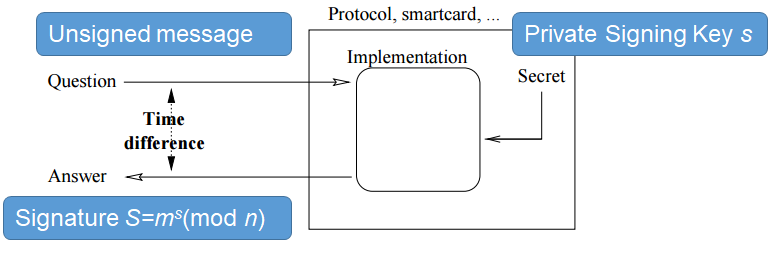
\includegraphics[scale=0.4]{images/smartcard.png}
    \caption{The timing attack principle} \label{fig:smart card}
\end{figure}

So, let's look a bit closer in the attack model, what messages we can send to the smart card? Can we send any message we want? The answer - we can only send valid messages, if the message is not valid the smart card will just throw them away. So, this is somewhere in the scale between the weakest model and the most powerful model. In this scenario the most permissive attack model is known plain text. Known plain text means that we can see the messages as they go in the smart card but cannot change them. So the next thing is chosen plain text, we can't  just chose any plain text, it has to follow a certain rule. The next thing is completely chosen plain text which doesn't enforce any rules, and the last thing is adaptive plain text which means we can look at the response and we can think the next that we will send. So, what is the attack model, we send requests, the smart card is signing them, and we get the responses and also we know that the smart card is using Montgomery RSA because it is a reasonable assumption. So how to use it to extract the key? So we are going to use a method named ``Vaizata" method which can be found in the DPA handbook. This is a general way of performing a side channel attack using statistics. \newline

\underline{The ``Vaizata" Method}
\begin{itemize}
	\item Make a simple assumption about the implementation
	\item Guess a little part of the key
	\item Make hypothesis about the effect of the guess on the execution
	\item Classify the measurements according to the hypothesis
	\item If we guessed right, the classification will be statistically meaningful
\end{itemize}

How does it works? First, we make a simple assumption on the implementation, an assumption could be: We assume that the implementation run on software (the other possibility is the hardware) what does it gives us? Software is executed serially and in the hardware it's not the case. We can assume for example that the key is stored in a flash memory on the device, and every time we need to use the key you need to read the flash memory. How can we find that this is the case? How can we find first of all that a device is on the hardware or on the software? One way is to look at it, We can open the screws and look with a microscope, We can go to this wonderful website called ``I fixed it". They disassemble all sorts of devices and share this information. What is the sign that the device is using software? If there is an update on the firmware, because when it wakes up it needs to find out what software to run. We can say this device uses memory, We can also say things about when the device is doing the encryption. So let's assume the device under test is a remote controller. Inside the controller there is a secret key stored and also a counter. Whenever the button is pressed the remote controller constructs a package containing the serial number of the controller, the counter and whatever Boolean state of the button (which ever button was pressed). Then it sends it to a car and the car decrypts it. Why by the way do we need a serial number? Each ECU in the car has program to accept remote controls. So why do we need the counter? Without the counter an attacker can repeat a message sent from the remote controller to the car only by reading the messages and sending them again. What happens when you press the button and the car is in the train station? The counter in the remote controller is out of sync with the counter in the car, there is a window of counter values the car will accept, if its closed the car will open without complaining. If it's a little closed we will need to press the remote control twice and when the car will see consecutive values it will open, but if it is too far it won't open. let's assume We can find out when the controller is transmitting (it is a very intensive operation that takes battery life and also radiates). So we know the moment in time when it is transmitting, did the encryption happened before or after the transmitting? Answer: before. Let's assume that the counter stored in the memory, let's say we found the moment in time when the chip is reading from memory, did it happen before or after the encryption? Answer: after, because we need the counter to be included in the message that will be sent.We can also make more assumptions such as ``the AES uses an 8 bit data pack or 16 bit or 32 bit", some of these assumptions might be wrong but the ``vizata" method will help us to find out if they are wrong. 

So first of all We make a simple assumption, assume that the smart card is using left to right binary exponentiation using Montgomery and this is a very reasonable assumption because everybody is using this method. The next thing to do is recursively (or inductively) guess a little part of the key. if we guessed the whole password it would take us exponential time but if we could guess a small part of the key each time it would take a linear time. So, we will try guess small parts of the key first, maybe the simplest thing to explain is guessing one bit or a single character but lets say we are guessing a small part of the key. So now we know the beginning of the key and there is a little part we don't know. So the next step, we need to make a guess about what kind of an effect our guess is going to have on the computation. We can say, for example, if we will guess the bit correctly than something will happen to the computation, if we will guess this key bit correctly it will take more power/take longer time/connect to the network more often, some kind of phenomena we can measure. So, in our case what is the only thing we can measure? Answer: time. we assume that if there is a Montgomery reduction in the calculation of this bit than the entire computation is going to take a little more time.


SO what is going on here? There is a very large computation here, we were able to guess the beginning of it but not the end of it. Now we are going to classify the measurements according to our hypothesis, in this case two groups (with or without Montgomery computation). If we guessed correctly then it will take longer to the group we said it will take longer. If not, it might take less or more, we don't know. If we guessed correctly, the groups will have meaning, means will will be able to statistically tell apart the set of the measurements that will take a longer time and the set of measurements that will take less time. We are going to guess the left most bit of the key, there are only two options, most of the cases it will be 1. The next bit? 1 or 0. Now, we can simulate the running of this algorithm with our guess, not all the key but only the part we know and if there is going to be Montgomery reduction. So assume we have g, e and N. The device under test is calculating \(g^emodn\) where g came from? Supplied by the attacker. What about of e? secret we want to discover (\(e_t,e_{t-1},..,e_0\)) What about of N? public variable (known). The first thing it does, it enters the Montgomery representation. This information of how to enter the Montgomery representation is known to the attacker. It starts with g, then g becomes Mont(g), the attacker can also do it. First \(A=1\), than \(A=A*A\) the next thing is \(A=A*g\) because we know that the most significant bit is 1. The next step is \(A=A*A\), now what is next? It depends, if \(e_{t-1}\) = 0 then \(A=A*A\) (skipping to next bit). Else if \(e_{t-1}\) = 1 then \(A=A*g\). What happens next now we don't know. We can run both calculations, in particular we can find out if there was a reduction step in two optional operations. There are 4 option either one containing reduction step, neither or both. We can know exactly, assuming we make a guess on \(e_{t-1}\), if there is going to be an extra reduction step. We know enough to guess, if we guess correctly, we can know if there will be reduction step because we can calculate all the alternative options completely. So, lets do this now, we have many different g's, we have repeated this step many times, and for each of these g's we know if there is going to be an extra reduction step. So, now let's see how we do an attack using this. So, there is private key s, public key v and signing operation \(m^s mod n\). 

We begin the attack with a bag of messages, all of them are valid, and we send them to the device under test (DUT). The DUT signs these messages (k messages), and for each one of the messages we get a trace, which is the data we collected using the side channel attack in this case it is only the time. now we have a vector of size k and each element in the vector is the time it took to sign the message. Now, we are going to try to guess \(s_t,s_{t-1}\)  
\((s = s_t,s_{t-1},s_{t-2},…,s_0)\) and try to discover \(s_{t-2}\). 

So for each of the messages and each key guess we are going to simulate the computation as far as we already know and in addition for the parts of the key we don't know we are going to simulate twice, why? One with a 0 and one with a 1. We are going to find out where the extra reduction step happens. If the next bit is 0, some of the messages have extra reduction we classify the message into two bins, those who got extra reduction and those who didn't. But maybe the key is not 0 maybe its 1. So we can simulate the same thing with the next bit as 1, and find out different set of messages with an extra reduction step. We can't find what the bits are but we can make a guess and simulate on both 0 and 1. So, now we divide our traces into two groups in 2 different ways, if the next key bit is 0 \(m_1,m_2,m_4,m_5,m_7\) got extra reduction and \(m_3,m_6,m_8,m_9\) didn't. If the next key bit is 1: \(m_2,m_3,m_5,m_8\) got extra reduction and \(m_1,m_4,m_6,m_7,m_9\) didn't (see \Cref{fig:extraRed}). 


\begin{figure}[!ht]
    \centering
    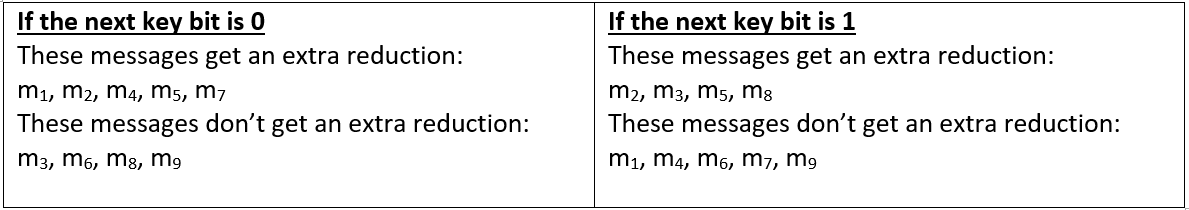
\includegraphics[scale=0.3]{images/extraRed.PNG}
    \caption{Key bit guess simulation} \label{fig:extraRed}
\end{figure}

If we guessed correctly what can we tell about the messages that got extra reduction? Answer: the runtime will be a little longer if we guessed the key bit correctly and If we guessed incorrectly it means we divided into two random groups which means the runtime will be similar in both groups. So if we guessed correctly the difference of runtime between the groups will be measurably different. So now we are going to change the discussion about the messages into the traces.

\begin{figure}[!ht]
    \centering
    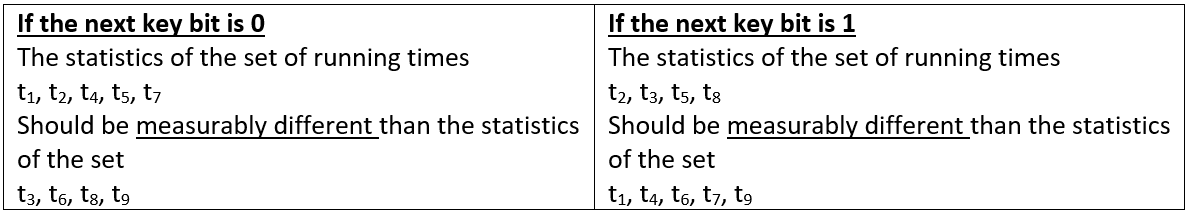
\includegraphics[scale=0.3]{images/extraStat.PNG}
    \caption{Guessing correctly the key bit makes the statics measurably different} \label{fig:extraStat}
\end{figure}


if the next key bit is 0 then the statistics of the runtimes of 0 bit with extra reduction are going to be different from the runtimes of 0 bit without extra reduction. If we guessed wrong the runtimes of 1 bit with extra reduction will be different from 1 bit without extra reduction. Notice that we are not saying average or mean anywhere, because they are not required, it could be the variance changes or something else, the point is that there is some kind of difference that we can measure. So, how can we find out which of these two divisions is the correct one? Answer: we have two divisions of k traces, we measure distance of means. We are going to calculate the mean runtime of each part (0 bit with or without the extra reduction and 1 bit with or without the extra reduction) and subtract between with/without extra reduction in each bit guess. If there is a large distance of means of the 0 bit guess as oppose to the 1 bit guess than probably the splitting of traces in the 0 bit guess is more meaningful than 1 bit guess, if we are able to split meaningfully then we guessed the key correctly. 
Now, let's go back into statistics and talk about the T-test~\cite{wikittest}. The T-test was invented by William Sealy Gosset~\cite{wikigosset} who was a chemist who worked for a very famous brewery in Ireland (Guinness). So, what is the idea? We have two populations that are different in some way. There are two kinds of t-tests, pair T-test and unpaired T-test. what is the paired T-test? lets assume we claim that we are going to a tree and we taking the leaves that fall off the tree. We notice that the leaves that fall on the south side have less mold that on the north side, why is that? Because there is more sun on the south side that is drying the leaves. 

How do we prove our theory? We send our undergrad research assistant to collect a bag of leaves form the north side and a bag of leaves from the south and now I tell the undergrad to count the percentage of mold in the southern and northern leaves. When the undergrad comes back, very exhausted, he provides us with an excel file that have 1000 leaves from the north side and 1500 from the south side. Now we want to prove our theory, each one of the leaves has a mold, We want to prove that there is a statistical difference between the two groups, this is the unpaired T-test. What is the paired? It is when we are talking about something which we can identify as pairs. For example, we are developing a cancer medicine and we want to test it. Now, we don't take any undergrads but only very sick mice with cancer. We measure the weight of the tumor in order to have a list of 100 mice and tumors. Then we divide them into two groups, one we treat with my medicine and the other we don't. In the end of the experiment, we measure the tumors again, but now each measurement is a pair, one before treatment and one is after. And we want to say that the size of the tumor is smaller after the treatment. 
Now let's review the student's unpaired T-test demo in Matlab. The mat in Matlab is for matrix, we can define matrix like this:

\begin{figure}[!ht]
    \centering
    \fbox{
    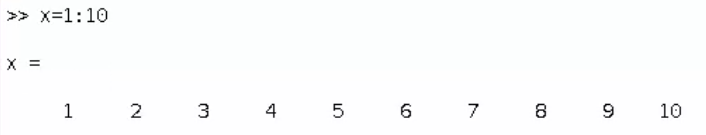
\includegraphics[scale=0.5]{images/defmat.png}}
    \caption{Defining a matrix of size 1x10 with increasing numbers from 1 [1,2,3,…,10]} \label{fig:defmat}
\end{figure}

\begin{figure}[!ht]
    \centering
    \fbox{
    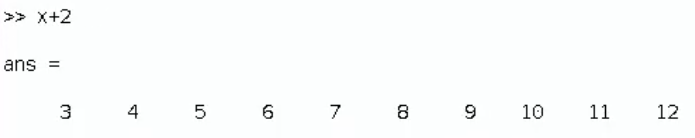
\includegraphics[scale=0.5]{images/defmat2.png}}
    \caption{Adding the matrix with 2 increases all the numbers in the matrix by 2 (Same with multiplication and log)} \label{fig:defmat2}
\end{figure}

\begin{figure}[!ht]
    \centering
    \fbox{
    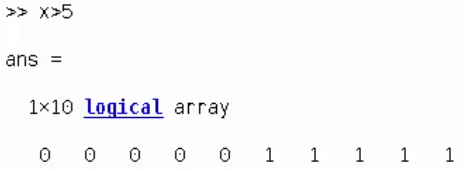
\includegraphics[scale=0.5]{images/defmat3.png}}
    \caption{\(x>5\) will result with logical array [0, 0, 0, 0…, 1, 1, 1, 1]} \label{fig:defmat3}
\end{figure}

The function randn(1) which creates normally distributed random variable which follows a Gaussian distribution which means the variance is 1 and the mean of 0. What is the minimum value this function will output? Answer: None, but statistically the value is closer to 0. How can we create a random variable with mean different from 0? Answer: add the mean, if we want mean N. we will do $N$ + randn (1). We can even create a vector of randomly chosen numbers using randn (1, 5) + 5 : [4.9369, 5.7147, 4.7950, 4.8759, 6.4897] and if we will do randn (1, 5)*.1 + 5 the numbers will be even closer to 5.
So, now we are ready to try the student T-test.

\begin{figure}[!ht]
    \centering
    \fbox{
    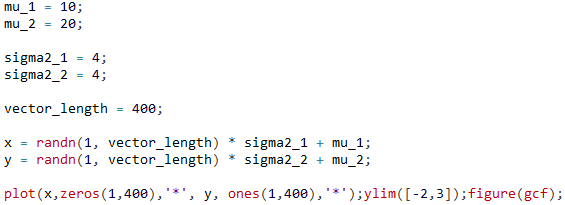
\includegraphics[scale=0.6]{images/defmat4.png}}
    \caption{In the code, 2 vectors are created - x and y in the same size (which is not obligatory), $x$ will be randomly distributed with a mean of \(mu_{1}\) and variance of \(sigma2_1\) and vector $x$ is going to be random distributed with a mean of \(mu_2\) and variance of \(sigma2_2\). Then there is a code for plotting both vectors (in different colors).} \label{fig:defmat4}
\end{figure}

\begin{figure}[!ht]
    \centering
    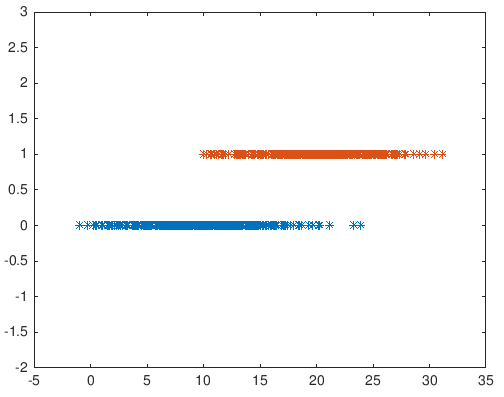
\includegraphics[scale=0.6]{images/defmatplot.png}
    \caption{Plotting of the vectors for \(mu_1 = 10, mu_2 = 20\)} \label{fig:defmatplot}
\end{figure}

Looking only on the graphs can we say they are from the same distribution? Answer: we can't be sure.
We want to run the T-test to find out if they are statistically significant. There is a hypothesis and we need to either reject or accept the hypothesis. If \(H_0\) than they are from the same distribution and if \(H_1\) than they are from different distributions. If we run the code the result will be that they are of different distributions with 0.959 certainty. Each time we ran we can get different results, if the certainty is smaller than 0.95 in matlab, the hypothesis is rejected. How can we make it more difficult for the ttest2? Answer: if we change \(mu_2\) to 11, than they will be very close distributions. 

\begin{figure}[!ht]
    \centering
    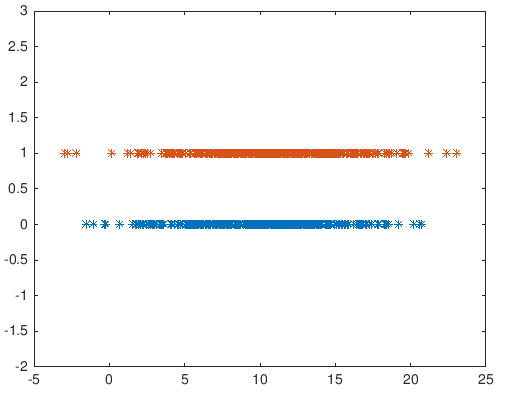
\includegraphics[scale=0.6]{images/defmatplot2.png}
    \caption{Plotting of the vectors for \(mu_1 = 10, mu_2 = 11\)} \label{fig:defmatplot2}
\end{figure}

How we as attackers will handle this situation? Answer: run many times. So we change the vector length (such as 50000). There is something called power analysis, which means given these parameters (mu and sigma) how many measurements you need to run to be sure with 95%.
As engineers we don't really care about T-tests, we have a budget of measurements and we just take the one with the larger mean distance, but what if we are wrong (guessed 1 instead of 0)? Answer: after we guessed one bit wrong all the bits afterwards are wrong because they are simulated wrongly.
So, how can we simulate a full attack? If we guessed 1 bit using the differences of means then we continue to the next bit in linear time. Lets review  a figure from " A Practical Implementation of the Timing Attack" which you are encouraged to read.


\begin{figure}[!ht]
    \centering
    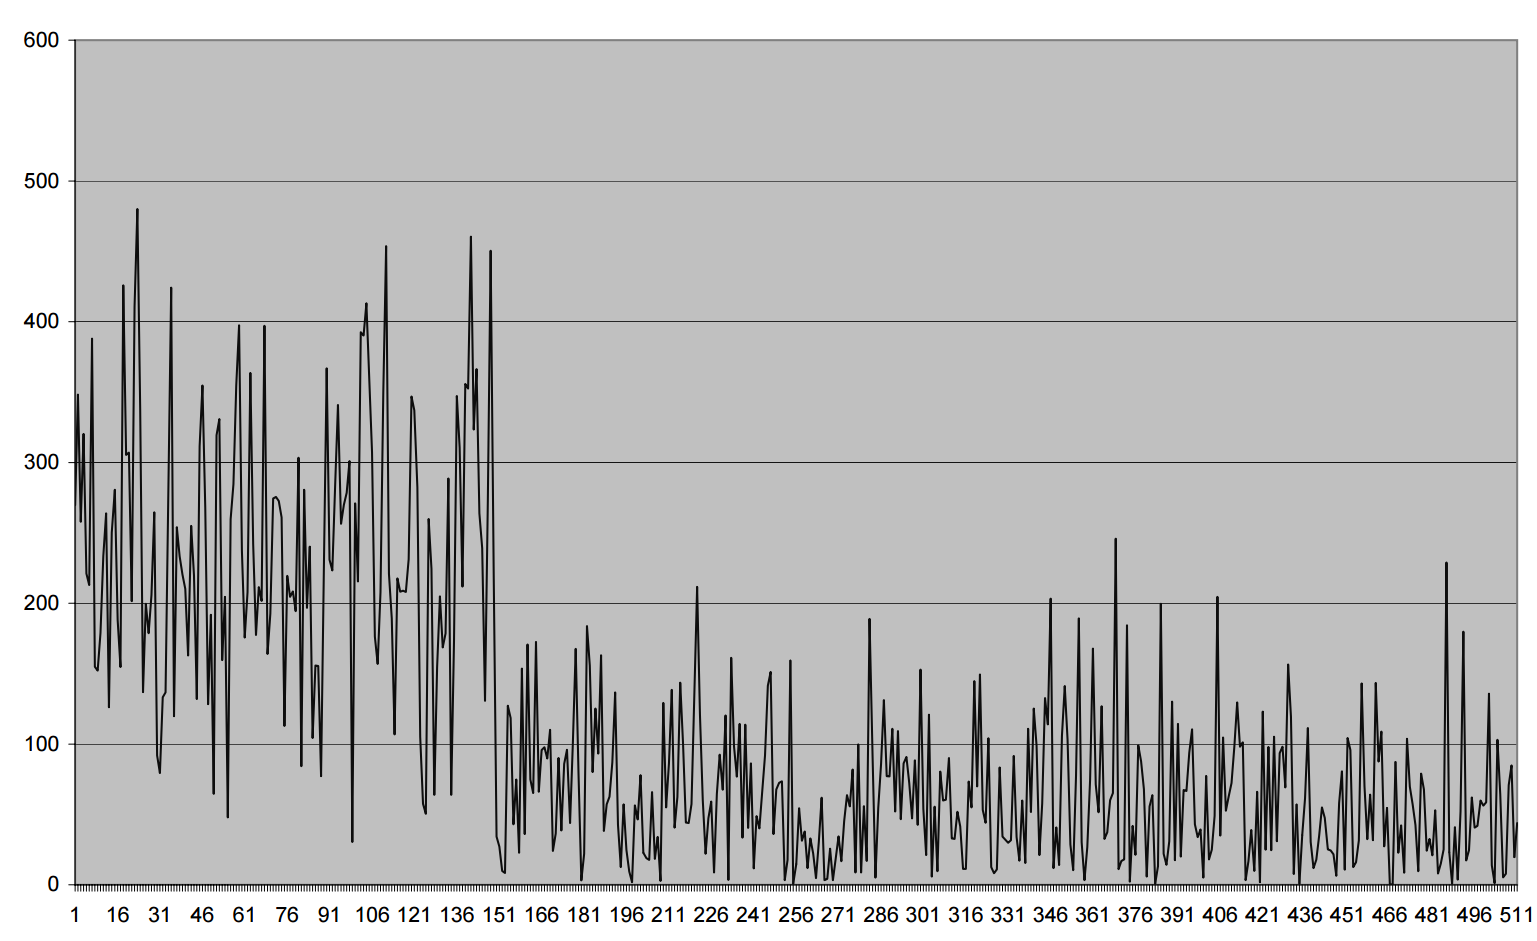
\includegraphics[scale=0.25]{images/figpita.png}
    \caption{x axis – is the bit index from right to left (the left most bit is known to be 1) and y axis – is the distance of means we chose (some times its 500 or 100 but after 151 the distance of means is a lot smaller which means we guessed a bit wrong). How to solve it? Answer: go backwards and backtrack.} \label{fig:figpita}
\end{figure}

Now lets talk about counter measurements. When Kocher announced the attack to the cipherpunks mailing list there was kind of discussion about it. Here is a message (see \Cref{fig:paul}) from there that was sent by Ron Riverst. He was replying to William Simpson, who was the author of Photuris which is related to the IPsec protocol and was used for kits change in the IP protocol. 

\begin{figure}[!ht]
    \centering
    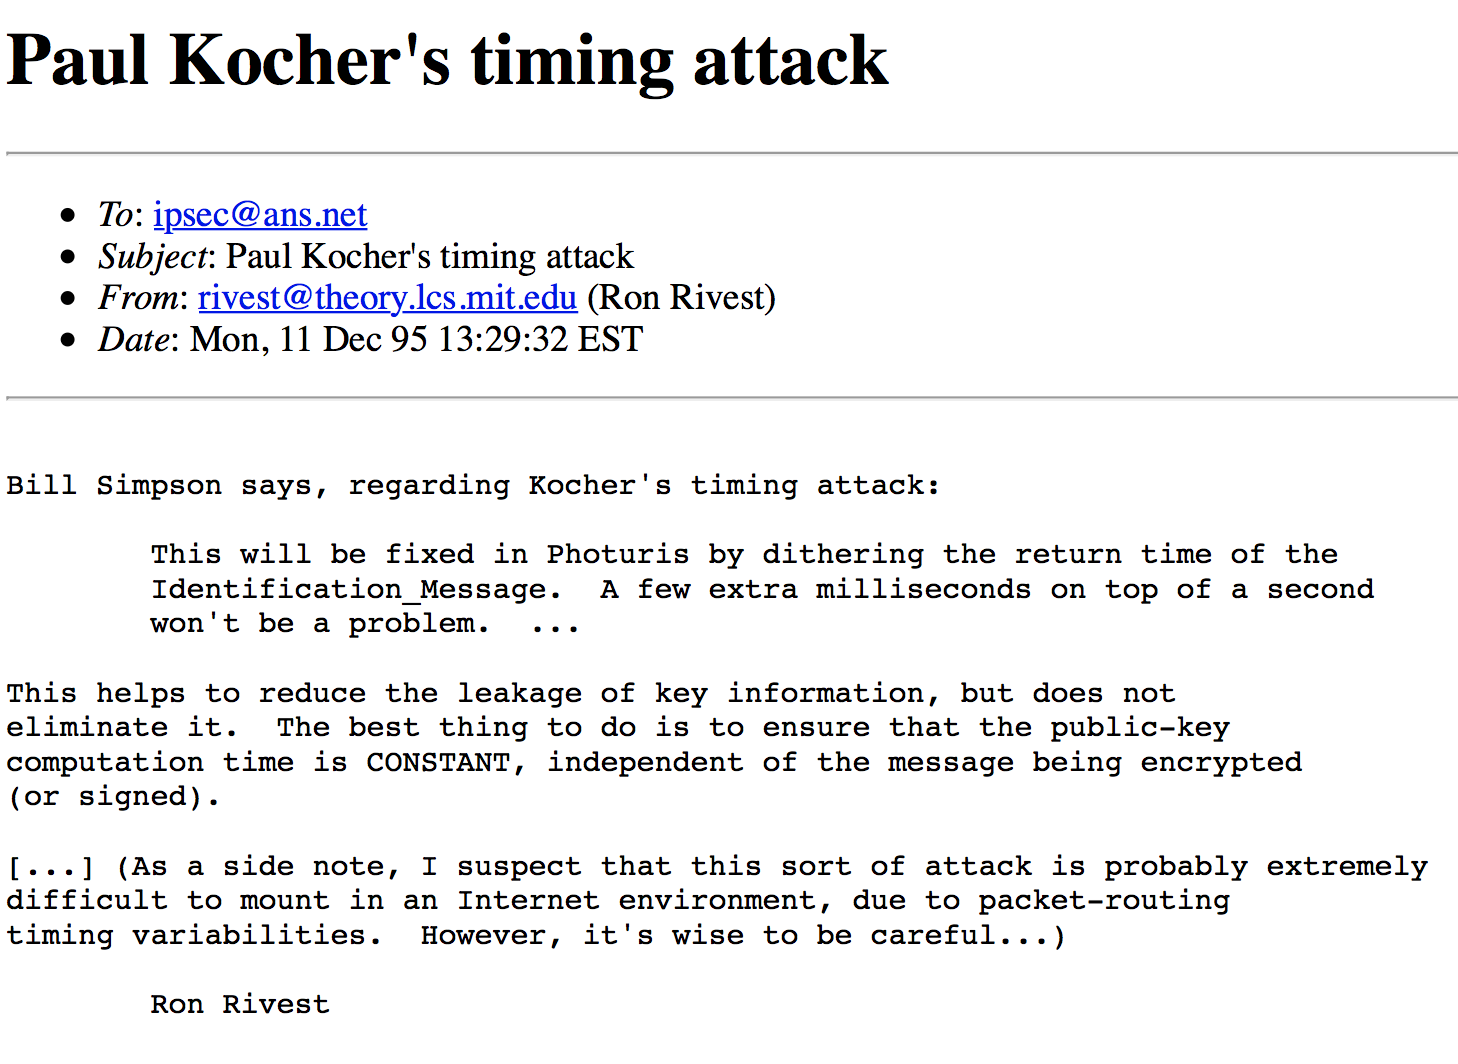
\includegraphics[scale=0.25]{images/paul.png}
    \caption{The message.} \label{fig:paul}
\end{figure}

When he read that this attack can attack Photuris, Bill replied: don't worry this will be fixed in Photuris. How to do this? By dithering the return time of identification message a few extra milliseconds. Which means he is doing mitigation, he is not adding a random delay because random is very expensive, he is going to finish the calculations and is going to look at the clock and exactly when the millisecond changes (or second) send the package. What does it mean? It means that since the beginning is random then he is going to add random delay. So, what Ron Rivest replied? It will reduce the data leakage but will not eliminate it. Why so? How the attacker will overcome this? Answer: he will need to measure more, this is network-based protocol, the attacker can measure many more times. He says, in addition, the public key computation time should be constant and independent from the message being sent. Ron Rivest suggest prevention as a countermeasure. So, what time it is going to be? Answer: the worst-case time. he adds a side note that this kind of attack is very difficult to mount in an internet environment due to packet-routing timing variabilities, however it is wise to be careful. Few years later a demonstration was presented over the internet, there were more measurements to counter the routing problem. Adding noise is sometimes the only thing that works, sometimes it works sometimes it doesn't, if you add enough noise to delay the attack time up to a year the message might not be relevant by the time the attack succeeds.

So, lets talk about two counter measurements, which are preventions. The first one is called RSA blinding. RSA blinding is a prevention counter measure which actually works on average time and not worst-case time. we have secret key S and want to calculate \(m^s mod n\), and the attacker gives us m and we don't want to leak s. We showed that with enough m from the attacker he will successfully retrieve s. 

So, how do we do blinding? First of all, we can do this even before the attacker arrives, we generate random $r$ and calculate \(r^v mod n\) and \(r^{-1} mod n\). these calculations are not reviling any secrets because v is the public key. The attacker gives us m, so we calculate: 

\[X = (r^v * m) mod n\]
\[Y = X^s = (r^v*m)^s = r^{vs}*m^s = r*m^s mod n \] 
\[ // v*s mod n = 1 mod n)\]

Now, $Y$ is leaking information because we raise a number to the power of the secret key, but $r$ is random number which the attacker doesn't know so he can't simulate the execution. How we remove r? We just calculate 

\[S = Y*r^{-1} = r*m^s*r^{-1} = m^s mod n\]

Why doesn't everybody use it? Answer: because its expensive, 2 modular exponentiations instead of 1. Another problem is the random number generation, its hard to find random number generator. You can see RSA blinding in openPGP. 

Now lets review another countermeasure. It called square and always multiply (see \Cref{fig:saama}). It is very similar to the square and multiply, just instead of only when \(d_i\) is 1 we will always calculate the multiply but the assignment will be only when \(d_i\) is 1. The problem with this is not the extra computation that came from turning sometimes to always. Speculative execution is always looking for instruction to execute, how does it decide if it will execute an instruction? If all its dependencies are met. If I say \(a = b*c\) and \(e = b*c\) they can run both in the same time. what happens is when the instruction brought to the CPU there is actually nobody is waiting for t, so as soon as it finishes to run the \(s =s *s mod n\) and \(d_i\) is equal to 0 it will just return s. Moreover, the compilers are also capable of detecting such cases and optimize them by dismissing the else statement. So if we have a very simple CPU with no speculative execution no compiler and we wrote it in assembly we wont be able to attack it, but we could use power analysis.

\begin{figure}[!ht]
    \centering
    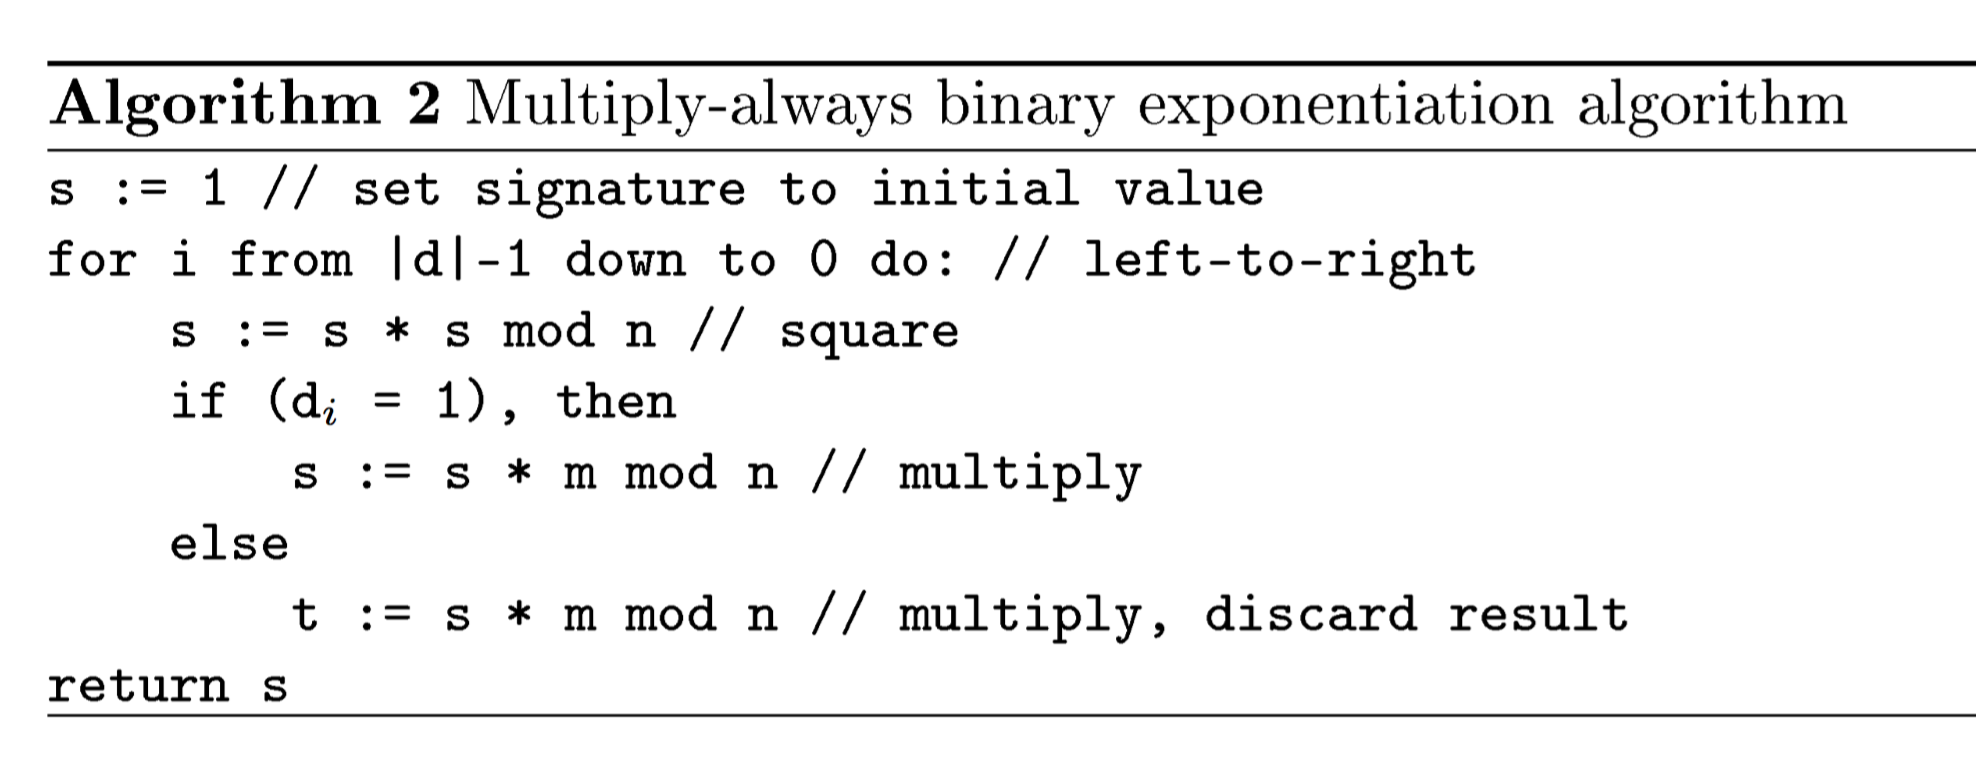
\includegraphics[scale=0.15]{images/saama.png}
    \caption{Square and always multiple algorithm} \label{fig:saama}
\end{figure}

If we run this algorithm as is, we have two places in memory for s and for t, every action we load s then multiply and then edit the memory of s, same goes in the multiply section. We load s and m then multiply and then store it in s. It's always loading and storing s, but what happens when it goes to the else segment: it loads s loads m and then store into something other then s. So the power consumption is different between the store and the load. You can read more in the paper (``defeating RSA multiply-always and message binding" by Marc F. Witteman et al.~\cite{witteman2011defeating})

Side channel attacks can get not only computer secrets but human secrets too. What exactly is a human secret? Browsing history for example. How does the website figure out our browsing history? Theoretically, we can delete the history in the browser. But what happens when we click on a hyper link (blue link)? It turns purple after the click. So, there was a nice trick that websites used to do, they attached the link to an HTML element and added JavaScript code that at the change of the color can now update that you have visited the site. The world wide web consortium decide that it was a privacy leak and you are not allowed to read the color of an HTML element anymore. Now we can set the color but can't read it. One of the speakers in the black hat 2013 used timing attacks to find out if a web site was visited or not\footnote{\url{https://www.youtube.com/watch?v=KcOQfYlyIqw}}. He also demonstrated how he can also use timing attack to read the user's stream. 